\section{Auswertung}
\label{sec:Auswertung}

Für die Auswertung wird die Python-Bibliothek \texttt{numpy} benutzt. Die Fits entstehen mit \texttt{curve\_fit} aus \texttt{scipy.optimize}.
Die Fehlerrechnung wird mit \texttt{uncertainties} durchgeführt. Plots entstehen mit \texttt{matplotlib.pyplot}. \\
Vor den Messreihen der beiden Pumpen wird der Rezipient lang genug evakuiert, sodass man einen angenäherten Enddruck $p_\text{E}$ messen kann. \\
Die Evakuierungskurven werden mit mehreren linearen Fits der Form
\begin{equation}
    y = m \cdot x + b
\end{equation}
über die Werte
\begin{equation}
    \ln{\frac{p(t) - p_\text{E}}{p_0 - p_\text{E}}} = -\frac{S}{V}t
    \label{eq:linfit}
\end{equation}
berechnet, sodass die verschiedenen Saugvermögen in den unterschiedlichen Druckbereichen über
\begin{equation}
    S = -m \cdot V
    \label{eq:S_evak}
\end{equation}
berechnet werden können. Dabei ist $m$ die Steigung in $\si{\milli\bar\per\second}$ und $b$ der $y$-Achsenabschnitt in $\si{\milli\bar}$. Im Folgenden werden die Einheiten bei der Angabe dieser Parameter ausgelassen.\\
Bei den Leckratenmessungen wird das Saugvermögen ebenfalls durch einen linearen Fit bestimmt.
$S$ ist hierbei gegeben durch
\begin{equation}
    S = m \cdot \frac{V}{p_\text{G}}
    \label{eq:S_leck}
\end{equation}

\subsection{Drehschieberpumpe}

Der für die Drehschieberpumpe nach einer ungefähr 30 minütigen Mittagspause gemessene Enddruck beträgt
\begin{equation}
    p_\text{E} = (\num{3.83} \pm \num{0.38}) \cdot 10^{-3} \, \si{\milli\bar}.\\
\end{equation}
Das Volumen wird der Versuchsanleitung entnommen und beträgt
\begin{equation}
    V_\text{Drehschieberpumpe} = (\num{34} \pm \num{3.4}) \, \si{\liter}.
\end{equation}


\subsubsection{Evakuierungskurve}

Für die Evakuierungskurve ergibt sich folgender Plot.

\begin{figure}[H]
    \centering
    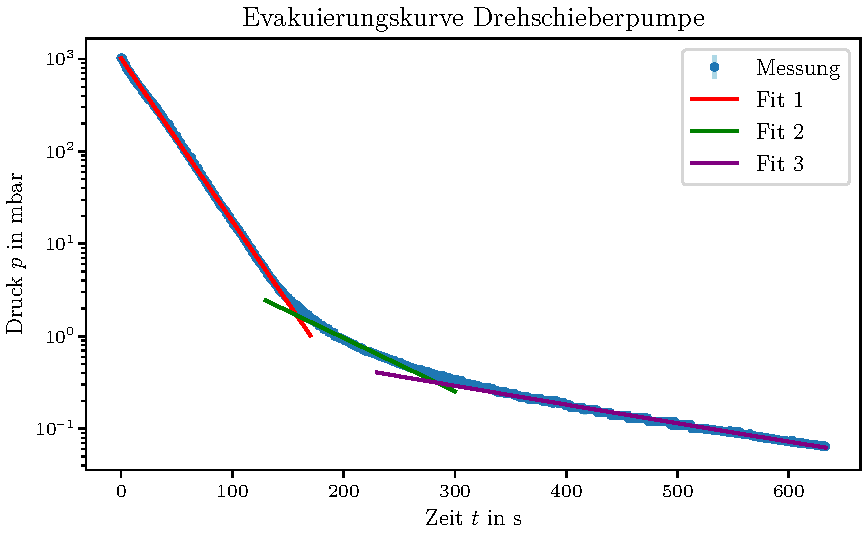
\includegraphics[width=\textwidth]{plots/DP_Evakuierungskurve.pdf}
    \caption{Es werden drei lineare Fits gemacht. Fit 1: $m = \num{-0.0408} \pm \num{0.0007}$, $b = \num{0.01} \pm \num{0.07}$. Fit 2: $m = \num{-0.01441} \pm \num{0.00034}$, $b = \num{-4.16} \pm \num{0.08}$. Fit 3: $m = \num{-0.00597} \pm \num{0.000004}$, $b = \num{-6.174} \pm \num{0.006}$.}
    \label{fig:DP_evak}
\end{figure}

Nach \eqref{eq:S_evak} finde man
\begin{align}
    S_1 &= (\num{1.39} \pm \num{0.14}) \si{\liter\per\second} \\
    S_2 &= (\num{0.49} \pm \num{0.05}) \si{\liter\per\second} \\
    S_3 &= (\num{0.41} \pm \num{0.04}) \si{\liter\per\second} 
\end{align}

$S_1$ hat dabei einen Gültigkeitsbereich von ungefähr $\SI{1000}{\milli\bar}$ bis ungefähr $\SI{2}{\milli\bar}$, $S_2$ von $\SI{2}{\milli\bar}$ bis $\SI{0.3}{\milli\bar}$ und $S_3$ darunter.

\subsubsection{Leckratenmessungen für bestimmte Gleichgewichtsdrücke $p_\text{G}$}

Für $p_\text{G} = \SI{100}{\milli\bar}$ werden drei Messungen gemacht und ein Mittelwert ausgewertet. Die anderen Gleichgewichtsdrücke werden nur einmal vermessen, da die statistische Abweichung ausreichend gering ist.

Es können folgende Messungen für $\SI{100}{\milli\bar}$ dargestellt werden.

\begin{figure}[H]
    \centering
    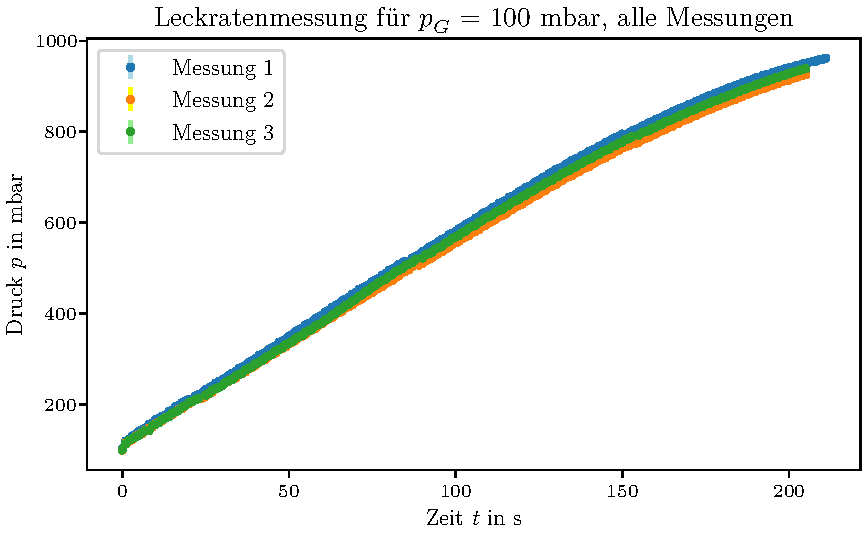
\includegraphics[width=\textwidth,height=8cm]{plots/DP_Leck_100mbar_alle.pdf}
    \caption{Alle drei Leckratenmessungen.}
    \label{fig:DP_leck_100mbar_alle}
\end{figure}

Für den Mittelwert ergibt sich folgende Grafik.

\begin{figure}[H]
    \centering
    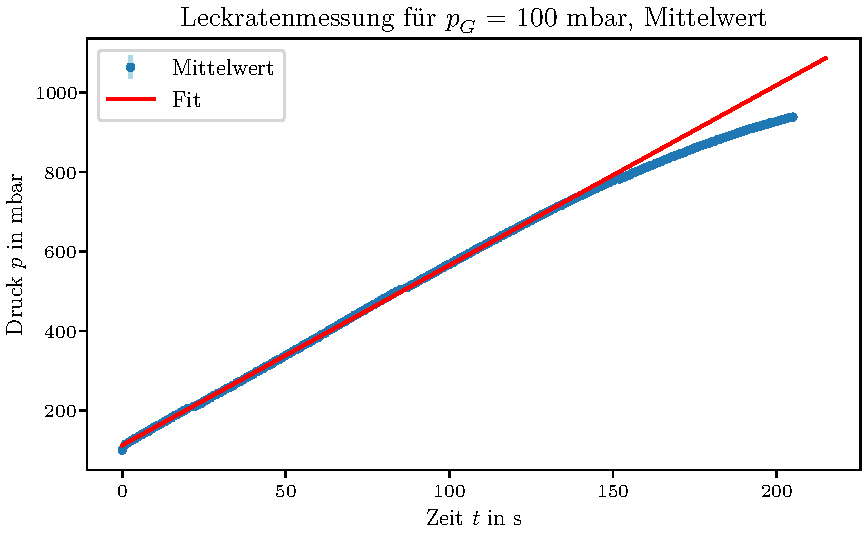
\includegraphics[width=\textwidth,height=8cm]{plots/DP_Leck1_100mbar_mittelwert.pdf}
    \caption{Mittelwerte der drei Messreihen. Fit: $m = \num{4.5283} \pm \num{0.0003}$, $b = \num{112.640} \pm \num{0.018}$.}
    \label{fig:DP_Leck_100mbar_mittelwert}
\end{figure}

Es ergibt sich ein Saugvermögen von
\begin{equation}
    S_{100} = (\num{1.54} \pm \num{0.16}) \si{\liter\per\second}.
\end{equation}

Für $p_\text{G} = \SI{50}{\milli\bar}$ ergibt sich folgende Grafik.

\begin{figure}[H]
    \centering
    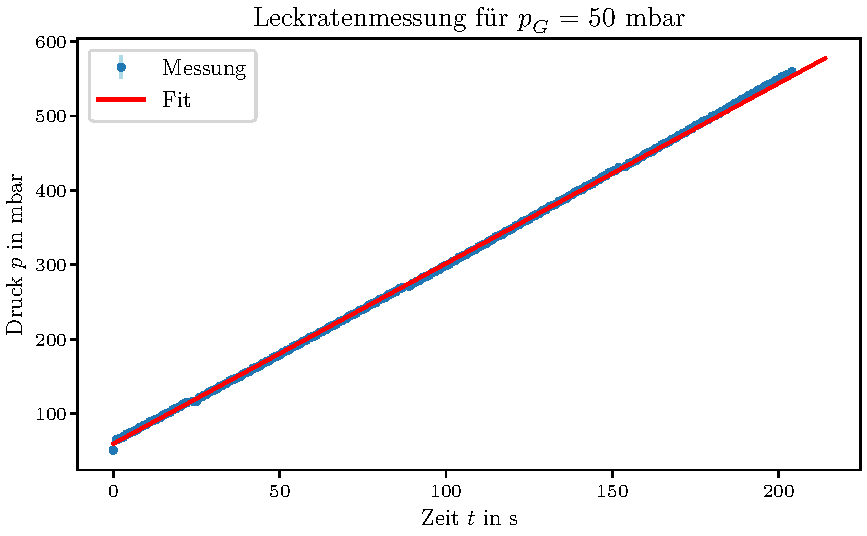
\includegraphics[width=\textwidth,height=8cm]{plots/DP_Leck_50mbar.pdf}
    \caption{Mittelwerte der drei Messreihen. Fit: $m = \num{2.419} \pm \num{0.001}$, $b = \num{59.78} \pm \num{0.07}$.}
    \label{fig:DP_Leck_50mbar_mittelwert}
\end{figure}

Es ergibt sich ein Saugvermögen von
\begin{equation}
    S_{50} = (\num{1.64} \pm \num{0.17}) \si{\liter\per\second}.
\end{equation}

Für $p_\text{G} = \SI{10}{\milli\bar}$ ergibt sich folgende Grafik.

\begin{figure}[H]
    \centering
    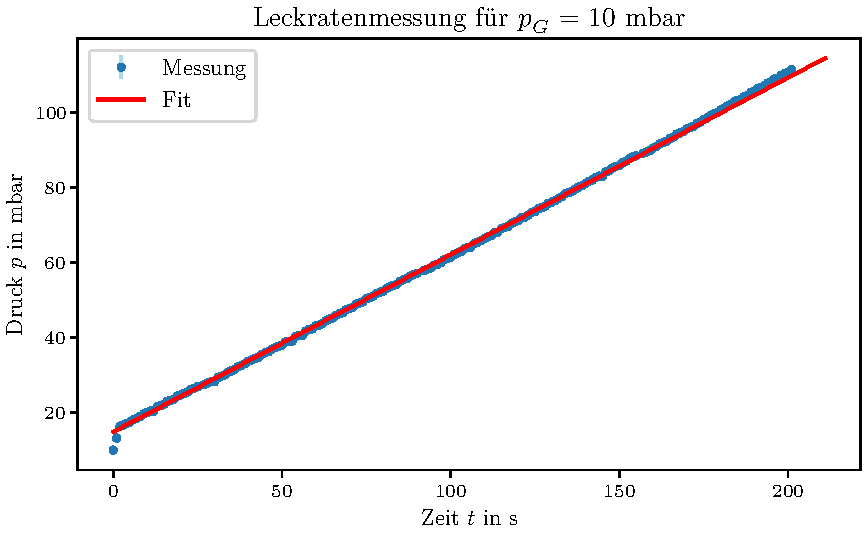
\includegraphics[width=\textwidth,height=8cm]{plots/DP_Leck_10mbar.pdf}
    \caption{Mittelwerte der drei Messreihen. Fit: $m = \num{0.47184} \pm \num{0.00022}$, $b = \num{14.886} \pm \num{0.016}$.}
    \label{fig:DP_Leck_10mbar_mittelwert}
\end{figure}

Es ergibt sich ein Saugvermögen von
\begin{equation}
    S_{10} = (\num{1.60} \pm \num{0.17}) \si{\liter\per\second}.
\end{equation}

Für $p_\text{G} = \SI{0.5}{\milli\bar}$ ergibt sich folgende Grafik.

\begin{figure}[H]
    \centering
    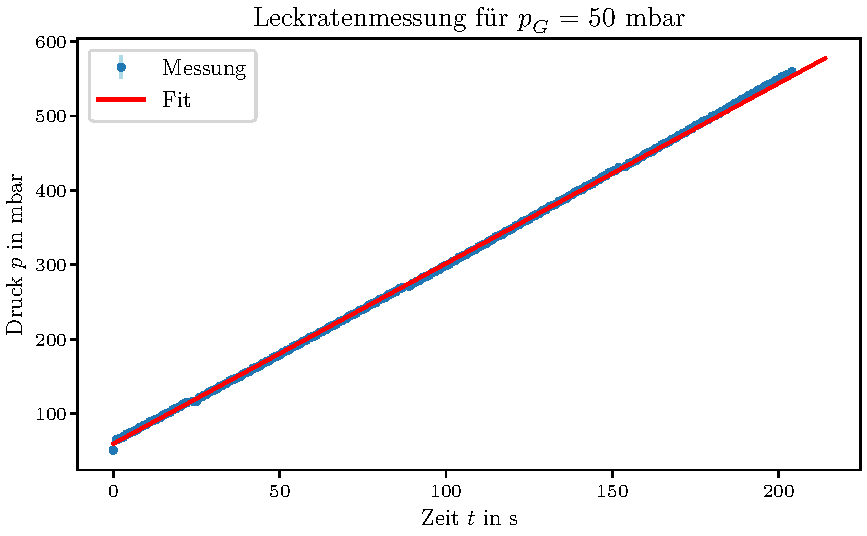
\includegraphics[width=\textwidth,height=8cm]{plots/DP_Leck_50mbar.pdf}
    \caption{Mittelwerte der drei Messreihen. Fit: $m = \num{0.0150} \pm \num{0.0004}$, $b = \num{1.63} \pm \num{0.04}$.}
    \label{fig:DP_Leck_05mbar_mittelwert}
\end{figure}

Es ergibt sich ein Saugvermögen von
\begin{equation}
    S_{\num{0.5}} = (\num{1.02} \pm \num{0.15}) \si{\liter\per\second}.
\end{equation}

\subsection{Turbomolekularpumpe}

Der für die Turbomolekularpumpe gemessene Enddruck beträgt
\begin{equation}
    p_\text{E} = (\num{5.0} \pm \num{1.5}) \cdot 10^{-5} \, \si{\milli\bar}.\\
\end{equation}
Das Volumen wird der Versuchsanleitung entnommen und beträgt
\begin{equation}
    V_\text{Drehschieberpumpe} = (\num{33} \pm \num{3.3}) \, \si{\liter}.
\end{equation}

\subsubsection{Evakuierungskurve}
Für die Evakuierungskurve werden drei Messreihen aufgenommen, bei der der Rezipient von einem Startdruck von ungefähr $p_0 = \num{5} \dot 10^{-5} \, \si{\milli\bar}$ evakuiert wird.
Diese sehen wie folgt aus.

\begin{figure}[H]
    \centering
    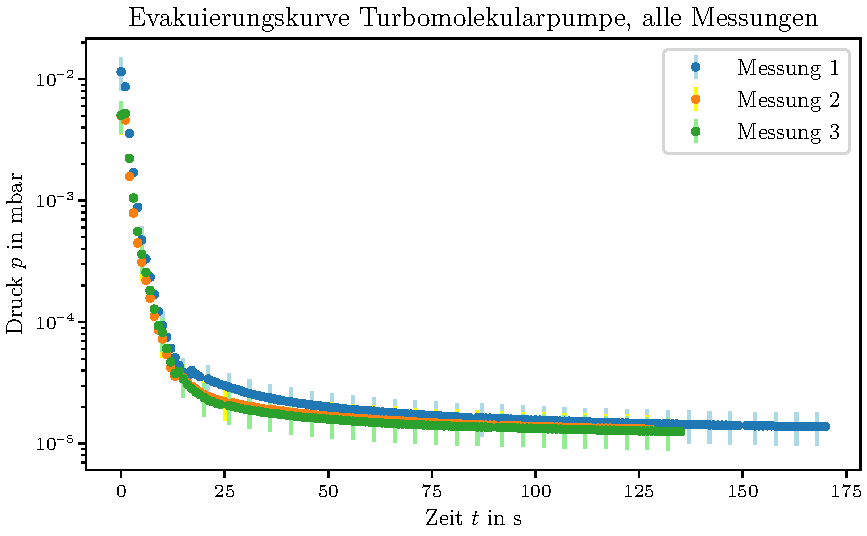
\includegraphics[width=\textwidth]{plots/TP_Evakuierungskurve_alle.pdf}
    \caption{Alle Evakuierungskurven.}
    \label{fig:TP_evak_alle}
\end{figure}

Alle Kurven haben einen kleinen Sprung, die blaue Kurve bei ungefähr $t = \SI{20}{\second}$, die grüne und orangene bei $t = \SI{15}{\second}$.
Für die Mittelwertbildung wird die blaue Kurve ignoriert. \\
Es ergibt sich folgende Grafik.

\begin{figure}[H]
    \centering
    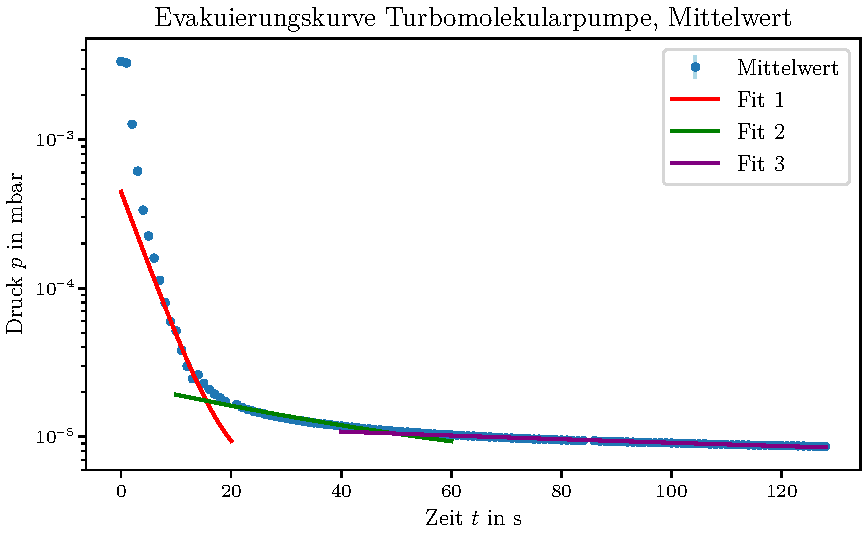
\includegraphics[width=\textwidth]{plots/TP_Evakuierungskurve.pdf}
    \caption{Es werden Fits gemacht. Fit 1: $m = \num{-0.2304202} \pm \num{0.0000004}$, $b = \num{2.030883} \pm \num{0.000005}$. Fit 2: $m = \num{-0.023777365} \pm \num{0.000000013}$, $b = \num{-5.2276858} \pm \num{0.0000005}$. Fit 3: $m = \num{0.0058313180} \pm \num{0.0000000027}$, $b = \num{-6.12055098} \pm \num{0.00000026}$.}
    \label{fig:TP_evak}
\end{figure}

